% Created by tikzDevice version 0.12.3 on 2019-09-26 18:24:11
% !TEX encoding = UTF-8 Unicode
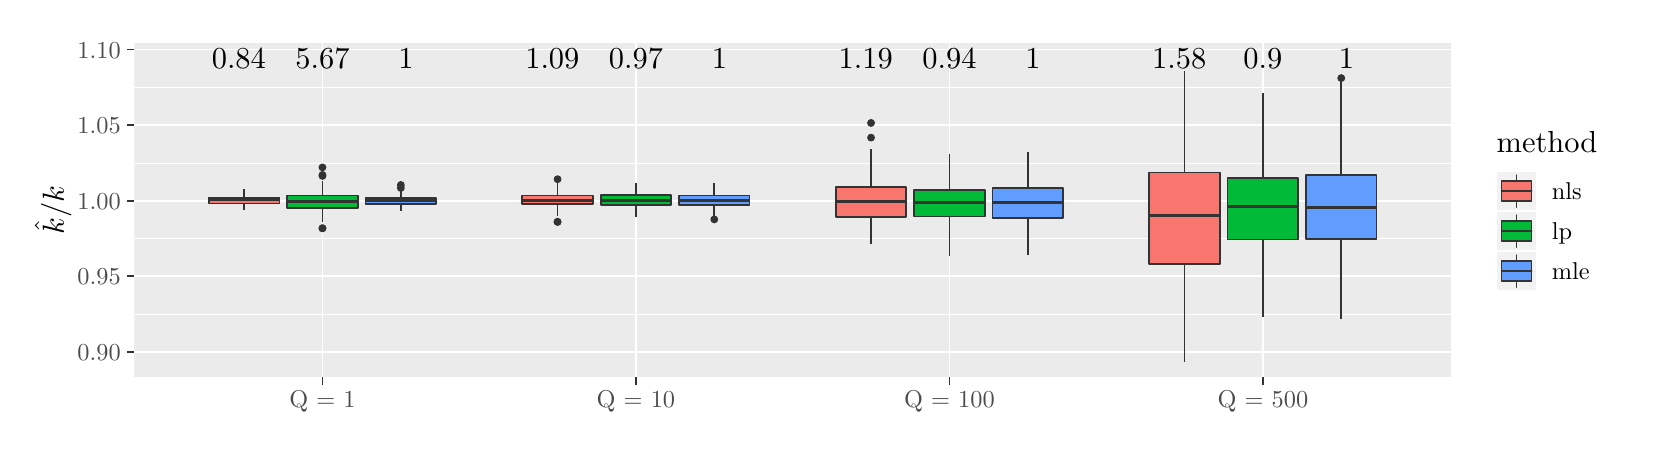
\begin{tikzpicture}[x=1pt,y=1pt]
\definecolor{fillColor}{RGB}{255,255,255}
\path[use as bounding box,fill=fillColor,fill opacity=0.00] (0,0) rectangle (578.16,144.54);
\begin{scope}
\path[clip] (  0.00,  0.00) rectangle (578.16,144.54);
\definecolor{drawColor}{RGB}{255,255,255}
\definecolor{fillColor}{RGB}{255,255,255}

\path[draw=drawColor,line width= 0.6pt,line join=round,line cap=round,fill=fillColor] (  0.00,  0.00) rectangle (578.16,144.54);
\end{scope}
\begin{scope}
\path[clip] ( 38.56, 18.22) rectangle (514.31,139.04);
\definecolor{fillColor}{gray}{0.92}

\path[fill=fillColor] ( 38.56, 18.22) rectangle (514.31,139.04);
\definecolor{drawColor}{RGB}{255,255,255}

\path[draw=drawColor,line width= 0.3pt,line join=round] ( 38.56, 41.07) --
	(514.31, 41.07);

\path[draw=drawColor,line width= 0.3pt,line join=round] ( 38.56, 68.36) --
	(514.31, 68.36);

\path[draw=drawColor,line width= 0.3pt,line join=round] ( 38.56, 95.65) --
	(514.31, 95.65);

\path[draw=drawColor,line width= 0.3pt,line join=round] ( 38.56,122.94) --
	(514.31,122.94);

\path[draw=drawColor,line width= 0.6pt,line join=round] ( 38.56, 27.43) --
	(514.31, 27.43);

\path[draw=drawColor,line width= 0.6pt,line join=round] ( 38.56, 54.72) --
	(514.31, 54.72);

\path[draw=drawColor,line width= 0.6pt,line join=round] ( 38.56, 82.01) --
	(514.31, 82.01);

\path[draw=drawColor,line width= 0.6pt,line join=round] ( 38.56,109.30) --
	(514.31,109.30);

\path[draw=drawColor,line width= 0.6pt,line join=round] ( 38.56,136.59) --
	(514.31,136.59);

\path[draw=drawColor,line width= 0.6pt,line join=round] (106.52, 18.22) --
	(106.52,139.04);

\path[draw=drawColor,line width= 0.6pt,line join=round] (219.79, 18.22) --
	(219.79,139.04);

\path[draw=drawColor,line width= 0.6pt,line join=round] (333.07, 18.22) --
	(333.07,139.04);

\path[draw=drawColor,line width= 0.6pt,line join=round] (446.34, 18.22) --
	(446.34,139.04);
\definecolor{drawColor}{gray}{0.20}

\path[draw=drawColor,line width= 0.6pt,line join=round] ( 78.20, 83.14) -- ( 78.20, 86.25);

\path[draw=drawColor,line width= 0.6pt,line join=round] ( 78.20, 80.97) -- ( 78.20, 78.72);
\definecolor{fillColor}{RGB}{248,118,109}

\path[draw=drawColor,line width= 0.6pt,line join=round,line cap=round,fill=fillColor] ( 65.46, 83.14) --
	( 65.46, 80.97) --
	( 90.94, 80.97) --
	( 90.94, 83.14) --
	( 65.46, 83.14) --
	cycle;

\path[draw=drawColor,line width= 1.1pt,line join=round] ( 65.46, 82.28) -- ( 90.94, 82.28);
\definecolor{fillColor}{gray}{0.20}

\path[draw=drawColor,line width= 0.4pt,line join=round,line cap=round,fill=fillColor] (106.52, 91.33) circle (  1.21);

\path[draw=drawColor,line width= 0.4pt,line join=round,line cap=round,fill=fillColor] (106.52, 90.96) circle (  1.21);

\path[draw=drawColor,line width= 0.4pt,line join=round,line cap=round,fill=fillColor] (106.52, 72.10) circle (  1.21);

\path[draw=drawColor,line width= 0.4pt,line join=round,line cap=round,fill=fillColor] (106.52, 72.01) circle (  1.21);

\path[draw=drawColor,line width= 0.4pt,line join=round,line cap=round,fill=fillColor] (106.52, 94.05) circle (  1.21);

\path[draw=drawColor,line width= 0.6pt,line join=round] (106.52, 83.86) -- (106.52, 89.20);

\path[draw=drawColor,line width= 0.6pt,line join=round] (106.52, 79.45) -- (106.52, 74.16);
\definecolor{fillColor}{RGB}{0,186,56}

\path[draw=drawColor,line width= 0.6pt,line join=round,line cap=round,fill=fillColor] ( 93.78, 83.86) --
	( 93.78, 79.45) --
	(119.26, 79.45) --
	(119.26, 83.86) --
	( 93.78, 83.86) --
	cycle;

\path[draw=drawColor,line width= 1.1pt,line join=round] ( 93.78, 81.79) -- (119.26, 81.79);
\definecolor{fillColor}{gray}{0.20}

\path[draw=drawColor,line width= 0.4pt,line join=round,line cap=round,fill=fillColor] (134.84, 86.61) circle (  1.21);

\path[draw=drawColor,line width= 0.4pt,line join=round,line cap=round,fill=fillColor] (134.84, 87.69) circle (  1.21);

\path[draw=drawColor,line width= 0.6pt,line join=round] (134.84, 82.93) -- (134.84, 85.76);

\path[draw=drawColor,line width= 0.6pt,line join=round] (134.84, 80.87) -- (134.84, 78.26);
\definecolor{fillColor}{RGB}{97,156,255}

\path[draw=drawColor,line width= 0.6pt,line join=round,line cap=round,fill=fillColor] (122.09, 82.93) --
	(122.09, 80.87) --
	(147.58, 80.87) --
	(147.58, 82.93) --
	(122.09, 82.93) --
	cycle;

\path[draw=drawColor,line width= 1.1pt,line join=round] (122.09, 81.95) -- (147.58, 81.95);
\definecolor{fillColor}{gray}{0.20}

\path[draw=drawColor,line width= 0.4pt,line join=round,line cap=round,fill=fillColor] (191.48, 74.35) circle (  1.21);

\path[draw=drawColor,line width= 0.4pt,line join=round,line cap=round,fill=fillColor] (191.48, 89.78) circle (  1.21);

\path[draw=drawColor,line width= 0.4pt,line join=round,line cap=round,fill=fillColor] (191.48, 74.39) circle (  1.21);

\path[draw=drawColor,line width= 0.6pt,line join=round] (191.48, 83.86) -- (191.48, 88.48);

\path[draw=drawColor,line width= 0.6pt,line join=round] (191.48, 80.77) -- (191.48, 76.41);
\definecolor{fillColor}{RGB}{248,118,109}

\path[draw=drawColor,line width= 0.6pt,line join=round,line cap=round,fill=fillColor] (178.73, 83.86) --
	(178.73, 80.77) --
	(204.22, 80.77) --
	(204.22, 83.86) --
	(178.73, 83.86) --
	cycle;

\path[draw=drawColor,line width= 1.1pt,line join=round] (178.73, 82.21) -- (204.22, 82.21);

\path[draw=drawColor,line width= 0.6pt,line join=round] (219.79, 84.06) -- (219.79, 88.49);

\path[draw=drawColor,line width= 0.6pt,line join=round] (219.79, 80.41) -- (219.79, 76.19);
\definecolor{fillColor}{RGB}{0,186,56}

\path[draw=drawColor,line width= 0.6pt,line join=round,line cap=round,fill=fillColor] (207.05, 84.06) --
	(207.05, 80.41) --
	(232.54, 80.41) --
	(232.54, 84.06) --
	(207.05, 84.06) --
	cycle;

\path[draw=drawColor,line width= 1.1pt,line join=round] (207.05, 82.04) -- (232.54, 82.04);
\definecolor{fillColor}{gray}{0.20}

\path[draw=drawColor,line width= 0.4pt,line join=round,line cap=round,fill=fillColor] (248.11, 75.26) circle (  1.21);

\path[draw=drawColor,line width= 0.6pt,line join=round] (248.11, 83.85) -- (248.11, 88.55);

\path[draw=drawColor,line width= 0.6pt,line join=round] (248.11, 80.48) -- (248.11, 75.83);
\definecolor{fillColor}{RGB}{97,156,255}

\path[draw=drawColor,line width= 0.6pt,line join=round,line cap=round,fill=fillColor] (235.37, 83.85) --
	(235.37, 80.48) --
	(260.86, 80.48) --
	(260.86, 83.85) --
	(235.37, 83.85) --
	cycle;

\path[draw=drawColor,line width= 1.1pt,line join=round] (235.37, 82.19) -- (260.86, 82.19);
\definecolor{fillColor}{gray}{0.20}

\path[draw=drawColor,line width= 0.4pt,line join=round,line cap=round,fill=fillColor] (304.75,104.81) circle (  1.21);

\path[draw=drawColor,line width= 0.4pt,line join=round,line cap=round,fill=fillColor] (304.75,110.11) circle (  1.21);

\path[draw=drawColor,line width= 0.6pt,line join=round] (304.75, 87.03) -- (304.75,100.54);

\path[draw=drawColor,line width= 0.6pt,line join=round] (304.75, 76.05) -- (304.75, 66.22);
\definecolor{fillColor}{RGB}{248,118,109}

\path[draw=drawColor,line width= 0.6pt,line join=round,line cap=round,fill=fillColor] (292.01, 87.03) --
	(292.01, 76.05) --
	(317.49, 76.05) --
	(317.49, 87.03) --
	(292.01, 87.03) --
	cycle;

\path[draw=drawColor,line width= 1.1pt,line join=round] (292.01, 81.78) -- (317.49, 81.78);

\path[draw=drawColor,line width= 0.6pt,line join=round] (333.07, 85.82) -- (333.07, 98.85);

\path[draw=drawColor,line width= 0.6pt,line join=round] (333.07, 76.29) -- (333.07, 61.99);
\definecolor{fillColor}{RGB}{0,186,56}

\path[draw=drawColor,line width= 0.6pt,line join=round,line cap=round,fill=fillColor] (320.33, 85.82) --
	(320.33, 76.29) --
	(345.81, 76.29) --
	(345.81, 85.82) --
	(320.33, 85.82) --
	cycle;

\path[draw=drawColor,line width= 1.1pt,line join=round] (320.33, 81.43) -- (345.81, 81.43);

\path[draw=drawColor,line width= 0.6pt,line join=round] (361.39, 86.69) -- (361.39, 99.52);

\path[draw=drawColor,line width= 0.6pt,line join=round] (361.39, 75.82) -- (361.39, 62.31);
\definecolor{fillColor}{RGB}{97,156,255}

\path[draw=drawColor,line width= 0.6pt,line join=round,line cap=round,fill=fillColor] (348.64, 86.69) --
	(348.64, 75.82) --
	(374.13, 75.82) --
	(374.13, 86.69) --
	(348.64, 86.69) --
	cycle;

\path[draw=drawColor,line width= 1.1pt,line join=round] (348.64, 81.24) -- (374.13, 81.24);

\path[draw=drawColor,line width= 0.6pt,line join=round] (418.02, 92.16) -- (418.02,128.86);

\path[draw=drawColor,line width= 0.6pt,line join=round] (418.02, 59.12) -- (418.02, 23.71);
\definecolor{fillColor}{RGB}{248,118,109}

\path[draw=drawColor,line width= 0.6pt,line join=round,line cap=round,fill=fillColor] (405.28, 92.16) --
	(405.28, 59.12) --
	(430.77, 59.12) --
	(430.77, 92.16) --
	(405.28, 92.16) --
	cycle;

\path[draw=drawColor,line width= 1.1pt,line join=round] (405.28, 76.61) -- (430.77, 76.61);

\path[draw=drawColor,line width= 0.6pt,line join=round] (446.34, 90.33) -- (446.34,120.90);

\path[draw=drawColor,line width= 0.6pt,line join=round] (446.34, 67.97) -- (446.34, 40.03);
\definecolor{fillColor}{RGB}{0,186,56}

\path[draw=drawColor,line width= 0.6pt,line join=round,line cap=round,fill=fillColor] (433.60, 90.33) --
	(433.60, 67.97) --
	(459.09, 67.97) --
	(459.09, 90.33) --
	(433.60, 90.33) --
	cycle;

\path[draw=drawColor,line width= 1.1pt,line join=round] (433.60, 79.92) -- (459.09, 79.92);
\definecolor{fillColor}{gray}{0.20}

\path[draw=drawColor,line width= 0.4pt,line join=round,line cap=round,fill=fillColor] (474.66,126.32) circle (  1.21);

\path[draw=drawColor,line width= 0.6pt,line join=round] (474.66, 91.28) -- (474.66,125.17);

\path[draw=drawColor,line width= 0.6pt,line join=round] (474.66, 68.08) -- (474.66, 39.41);
\definecolor{fillColor}{RGB}{97,156,255}

\path[draw=drawColor,line width= 0.6pt,line join=round,line cap=round,fill=fillColor] (461.92, 91.28) --
	(461.92, 68.08) --
	(487.40, 68.08) --
	(487.40, 91.28) --
	(461.92, 91.28) --
	cycle;

\path[draw=drawColor,line width= 1.1pt,line join=round] (461.92, 79.61) -- (487.40, 79.61);
\definecolor{drawColor}{RGB}{0,0,0}

\node[text=drawColor,anchor=base,inner sep=0pt, outer sep=0pt, scale=  1.10] at (136.73,129.75) {1};

\node[text=drawColor,anchor=base,inner sep=0pt, outer sep=0pt, scale=  1.10] at (106.52,129.75) {5.67};

\node[text=drawColor,anchor=base,inner sep=0pt, outer sep=0pt, scale=  1.10] at ( 76.31,129.75) {0.84};

\node[text=drawColor,anchor=base,inner sep=0pt, outer sep=0pt, scale=  1.10] at (250.00,129.75) {1};

\node[text=drawColor,anchor=base,inner sep=0pt, outer sep=0pt, scale=  1.10] at (219.79,129.75) {0.97};

\node[text=drawColor,anchor=base,inner sep=0pt, outer sep=0pt, scale=  1.10] at (189.59,129.75) {1.09};

\node[text=drawColor,anchor=base,inner sep=0pt, outer sep=0pt, scale=  1.10] at (363.28,129.75) {1};

\node[text=drawColor,anchor=base,inner sep=0pt, outer sep=0pt, scale=  1.10] at (333.07,129.75) {0.94};

\node[text=drawColor,anchor=base,inner sep=0pt, outer sep=0pt, scale=  1.10] at (302.86,129.75) {1.19};

\node[text=drawColor,anchor=base,inner sep=0pt, outer sep=0pt, scale=  1.10] at (476.55,129.75) {1};

\node[text=drawColor,anchor=base,inner sep=0pt, outer sep=0pt, scale=  1.10] at (446.34,129.75) {0.9};

\node[text=drawColor,anchor=base,inner sep=0pt, outer sep=0pt, scale=  1.10] at (416.14,129.75) {1.58};
\end{scope}
\begin{scope}
\path[clip] (  0.00,  0.00) rectangle (578.16,144.54);
\definecolor{drawColor}{gray}{0.30}

\node[text=drawColor,anchor=base east,inner sep=0pt, outer sep=0pt, scale=  0.88] at ( 33.61, 24.40) {0.90};

\node[text=drawColor,anchor=base east,inner sep=0pt, outer sep=0pt, scale=  0.88] at ( 33.61, 51.69) {0.95};

\node[text=drawColor,anchor=base east,inner sep=0pt, outer sep=0pt, scale=  0.88] at ( 33.61, 78.98) {1.00};

\node[text=drawColor,anchor=base east,inner sep=0pt, outer sep=0pt, scale=  0.88] at ( 33.61,106.27) {1.05};

\node[text=drawColor,anchor=base east,inner sep=0pt, outer sep=0pt, scale=  0.88] at ( 33.61,133.56) {1.10};
\end{scope}
\begin{scope}
\path[clip] (  0.00,  0.00) rectangle (578.16,144.54);
\definecolor{drawColor}{gray}{0.20}

\path[draw=drawColor,line width= 0.6pt,line join=round] ( 35.81, 27.43) --
	( 38.56, 27.43);

\path[draw=drawColor,line width= 0.6pt,line join=round] ( 35.81, 54.72) --
	( 38.56, 54.72);

\path[draw=drawColor,line width= 0.6pt,line join=round] ( 35.81, 82.01) --
	( 38.56, 82.01);

\path[draw=drawColor,line width= 0.6pt,line join=round] ( 35.81,109.30) --
	( 38.56,109.30);

\path[draw=drawColor,line width= 0.6pt,line join=round] ( 35.81,136.59) --
	( 38.56,136.59);
\end{scope}
\begin{scope}
\path[clip] (  0.00,  0.00) rectangle (578.16,144.54);
\definecolor{drawColor}{gray}{0.20}

\path[draw=drawColor,line width= 0.6pt,line join=round] (106.52, 15.47) --
	(106.52, 18.22);

\path[draw=drawColor,line width= 0.6pt,line join=round] (219.79, 15.47) --
	(219.79, 18.22);

\path[draw=drawColor,line width= 0.6pt,line join=round] (333.07, 15.47) --
	(333.07, 18.22);

\path[draw=drawColor,line width= 0.6pt,line join=round] (446.34, 15.47) --
	(446.34, 18.22);
\end{scope}
\begin{scope}
\path[clip] (  0.00,  0.00) rectangle (578.16,144.54);
\definecolor{drawColor}{gray}{0.30}

\node[text=drawColor,anchor=base,inner sep=0pt, outer sep=0pt, scale=  0.88] at (106.52,  7.21) {Q = 1};

\node[text=drawColor,anchor=base,inner sep=0pt, outer sep=0pt, scale=  0.88] at (219.79,  7.21) {Q = 10};

\node[text=drawColor,anchor=base,inner sep=0pt, outer sep=0pt, scale=  0.88] at (333.07,  7.21) {Q = 100};

\node[text=drawColor,anchor=base,inner sep=0pt, outer sep=0pt, scale=  0.88] at (446.34,  7.21) {Q = 500};
\end{scope}
\begin{scope}
\path[clip] (  0.00,  0.00) rectangle (578.16,144.54);
\definecolor{drawColor}{RGB}{0,0,0}

\node[text=drawColor,rotate= 90.00,anchor=base,inner sep=0pt, outer sep=0pt, scale=  1.10] at ( 13.08, 78.63) {$\hat{k}/k$};
\end{scope}
\begin{scope}
\path[clip] (  0.00,  0.00) rectangle (578.16,144.54);
\definecolor{fillColor}{RGB}{255,255,255}

\path[fill=fillColor] (525.31, 43.84) rectangle (572.66,113.42);
\end{scope}
\begin{scope}
\path[clip] (  0.00,  0.00) rectangle (578.16,144.54);
\definecolor{drawColor}{RGB}{0,0,0}

\node[text=drawColor,anchor=base west,inner sep=0pt, outer sep=0pt, scale=  1.10] at (530.81, 99.27) {method};
\end{scope}
\begin{scope}
\path[clip] (  0.00,  0.00) rectangle (578.16,144.54);
\definecolor{drawColor}{RGB}{255,255,255}
\definecolor{fillColor}{gray}{0.95}

\path[draw=drawColor,line width= 0.6pt,line join=round,line cap=round,fill=fillColor] (530.81, 78.25) rectangle (545.26, 92.70);
\end{scope}
\begin{scope}
\path[clip] (  0.00,  0.00) rectangle (578.16,144.54);
\definecolor{drawColor}{gray}{0.20}

\path[draw=drawColor,line width= 0.6pt,line join=round,line cap=round] (538.03, 79.70) --
	(538.03, 81.86);

\path[draw=drawColor,line width= 0.6pt,line join=round,line cap=round] (538.03, 89.09) --
	(538.03, 91.26);
\definecolor{fillColor}{RGB}{248,118,109}

\path[draw=drawColor,line width= 0.6pt,line join=round,line cap=round,fill=fillColor] (532.61, 81.86) rectangle (543.45, 89.09);

\path[draw=drawColor,line width= 0.6pt,line join=round,line cap=round] (532.61, 85.48) --
	(543.45, 85.48);
\end{scope}
\begin{scope}
\path[clip] (  0.00,  0.00) rectangle (578.16,144.54);
\definecolor{drawColor}{RGB}{255,255,255}
\definecolor{fillColor}{gray}{0.95}

\path[draw=drawColor,line width= 0.6pt,line join=round,line cap=round,fill=fillColor] (530.81, 63.80) rectangle (545.26, 78.25);
\end{scope}
\begin{scope}
\path[clip] (  0.00,  0.00) rectangle (578.16,144.54);
\definecolor{drawColor}{gray}{0.20}

\path[draw=drawColor,line width= 0.6pt,line join=round,line cap=round] (538.03, 65.24) --
	(538.03, 67.41);

\path[draw=drawColor,line width= 0.6pt,line join=round,line cap=round] (538.03, 74.64) --
	(538.03, 76.81);
\definecolor{fillColor}{RGB}{0,186,56}

\path[draw=drawColor,line width= 0.6pt,line join=round,line cap=round,fill=fillColor] (532.61, 67.41) rectangle (543.45, 74.64);

\path[draw=drawColor,line width= 0.6pt,line join=round,line cap=round] (532.61, 71.02) --
	(543.45, 71.02);
\end{scope}
\begin{scope}
\path[clip] (  0.00,  0.00) rectangle (578.16,144.54);
\definecolor{drawColor}{RGB}{255,255,255}
\definecolor{fillColor}{gray}{0.95}

\path[draw=drawColor,line width= 0.6pt,line join=round,line cap=round,fill=fillColor] (530.81, 49.34) rectangle (545.26, 63.80);
\end{scope}
\begin{scope}
\path[clip] (  0.00,  0.00) rectangle (578.16,144.54);
\definecolor{drawColor}{gray}{0.20}

\path[draw=drawColor,line width= 0.6pt,line join=round,line cap=round] (538.03, 50.79) --
	(538.03, 52.96);

\path[draw=drawColor,line width= 0.6pt,line join=round,line cap=round] (538.03, 60.18) --
	(538.03, 62.35);
\definecolor{fillColor}{RGB}{97,156,255}

\path[draw=drawColor,line width= 0.6pt,line join=round,line cap=round,fill=fillColor] (532.61, 52.96) rectangle (543.45, 60.18);

\path[draw=drawColor,line width= 0.6pt,line join=round,line cap=round] (532.61, 56.57) --
	(543.45, 56.57);
\end{scope}
\begin{scope}
\path[clip] (  0.00,  0.00) rectangle (578.16,144.54);
\definecolor{drawColor}{RGB}{0,0,0}

\node[text=drawColor,anchor=base west,inner sep=0pt, outer sep=0pt, scale=  0.88] at (550.76, 82.45) {nls};
\end{scope}
\begin{scope}
\path[clip] (  0.00,  0.00) rectangle (578.16,144.54);
\definecolor{drawColor}{RGB}{0,0,0}

\node[text=drawColor,anchor=base west,inner sep=0pt, outer sep=0pt, scale=  0.88] at (550.76, 67.99) {lp};
\end{scope}
\begin{scope}
\path[clip] (  0.00,  0.00) rectangle (578.16,144.54);
\definecolor{drawColor}{RGB}{0,0,0}

\node[text=drawColor,anchor=base west,inner sep=0pt, outer sep=0pt, scale=  0.88] at (550.76, 53.54) {mle};
\end{scope}
\end{tikzpicture}
